\begin{document}
	
	\section{Pipeline Description}
	
	The aim of these thesis is the developing of a pipeline for the identification of GGO and CS areas in chest CT scans of COVID-19 affected patients. The pipeline aims to have the following characteristics:   
	\begin{itemize}
		\item  \textbf{Fully Automated: } to remove the dependency from an external operator, and so the subjectivity of the segmentation; 
		
		\item \textbf{Fast: } in order to compete with certified software and to provides a segmentation in few minutes.
	\end{itemize}
	
	The segmentation of the lesion areas in made by unsupervised technique, se doesn't requires to provide hte expected outcomes. The whole pipeline was developed and tested on CT scans kindly provided by Sant'Orsola Hospital. Also the public datasets were used as benchmark. The used datasets are manually annotated; the provided labels are used to check the pipeline performances.\\ During the pipeline developing we have to takes into account is that the infection regions may have different patterns according to the stage of the disease or recovery, as we can see in \figurename\,\ref{fig:GGO-Spatial}, and usually these patterns are spatially disconnected; so we have decided to use a pixel classification technique.\\
	
	\begin{figure}[h!]
		\centering
			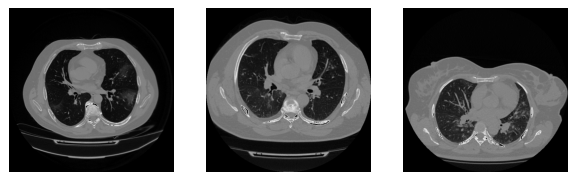
\includegraphics[scale=1.5]{GGOSeveralPatients.png}
		\caption{Groud Glass Opacity of COVID-19 affected patients with different severity of the disease. From left to right this scans belong to CT-1, CT-2 and CT-4 category of MOSMED~\cite{DATA:MOSMED} dataset}
	\label{fig:GGO-Spatial}
	\end{figure}

	The basic idea was to use the color quantization technique for the segmentation, grouping voxel based on color similarity, by assign  to each tissue a characteristic color. This can be done since in CT scan exist a relationship between the tissue in the voxel and the Gray Level used to display it, given by the Hounsfiend Units(eq\,\ref{eq:HU}: colors are proportional to HU, which are defined as a linear transformation of the linear attenuation coefficient($\mu$).
		
	Color quantization and the properties of digital images allow to consider also other properties of the image besides the single voxel intensity.
	As I've said before, in digital image processing, images are represented with a 3D tensor, in which the first two dimensions represent the height and width of the image  and the last one the number of channels. In this work the different channel are used to takes in account different properties, exploited by the application of different filters. This allow us to consider also neighboring voxels, that is really suitable for the segmentation since the  lesions areas involves many closest voxels, not only a single one. We have also used this features to discriminate between other lung regions like bronchi by exploit shape information.\\
	
	Once we have build the color space, we have to found the characteristic color of each tissue under study, which is represented by a centroids in the color space. In order to perform this task and achieve the centroids estimation a simple k-means clustering was used, since it provides a suitable segmentation with good time performances and it is efficiently implemented for multi-channel images in OpenCV~\cite{OpenCV}. 
	K-means clustering requires a prior knowledge about the number of cluster, which in our case is given by the anatomical structure of the lung, so we can consider a different cluster for each anatomical structure.\\
	Once we have estimated the centroids for each tissue, we use that for the actual segmentation, by assign each voxel to the cluster of the closest centroids: in this way the estimation step, that we will call "train", needs to be performed only once, so can be time expansive since is not involved in the actual segmentation.\\
	
\end{document}